\documentclass{article}

\usepackage{graphicx}

\usepackage{datetime}
\newdate{date}{08}{03}{2018}
\date{\displaydate{date}}

\title{Report}

\begin{document}

\maketitle

After reading papers on the subject, I identified the PDB structure 1G3X as the first system to calculate the binding affinity of. It is $[d(CGCGAATTCGCG)]_2$ double stranded DNA, with the planar aromatic intercalator 9-acridine.

Today (Friday) I will be parametrising the system. Once it is ready for simulation I will write down the exact protocol used.

See next page for more detail.

\begin{figure}
  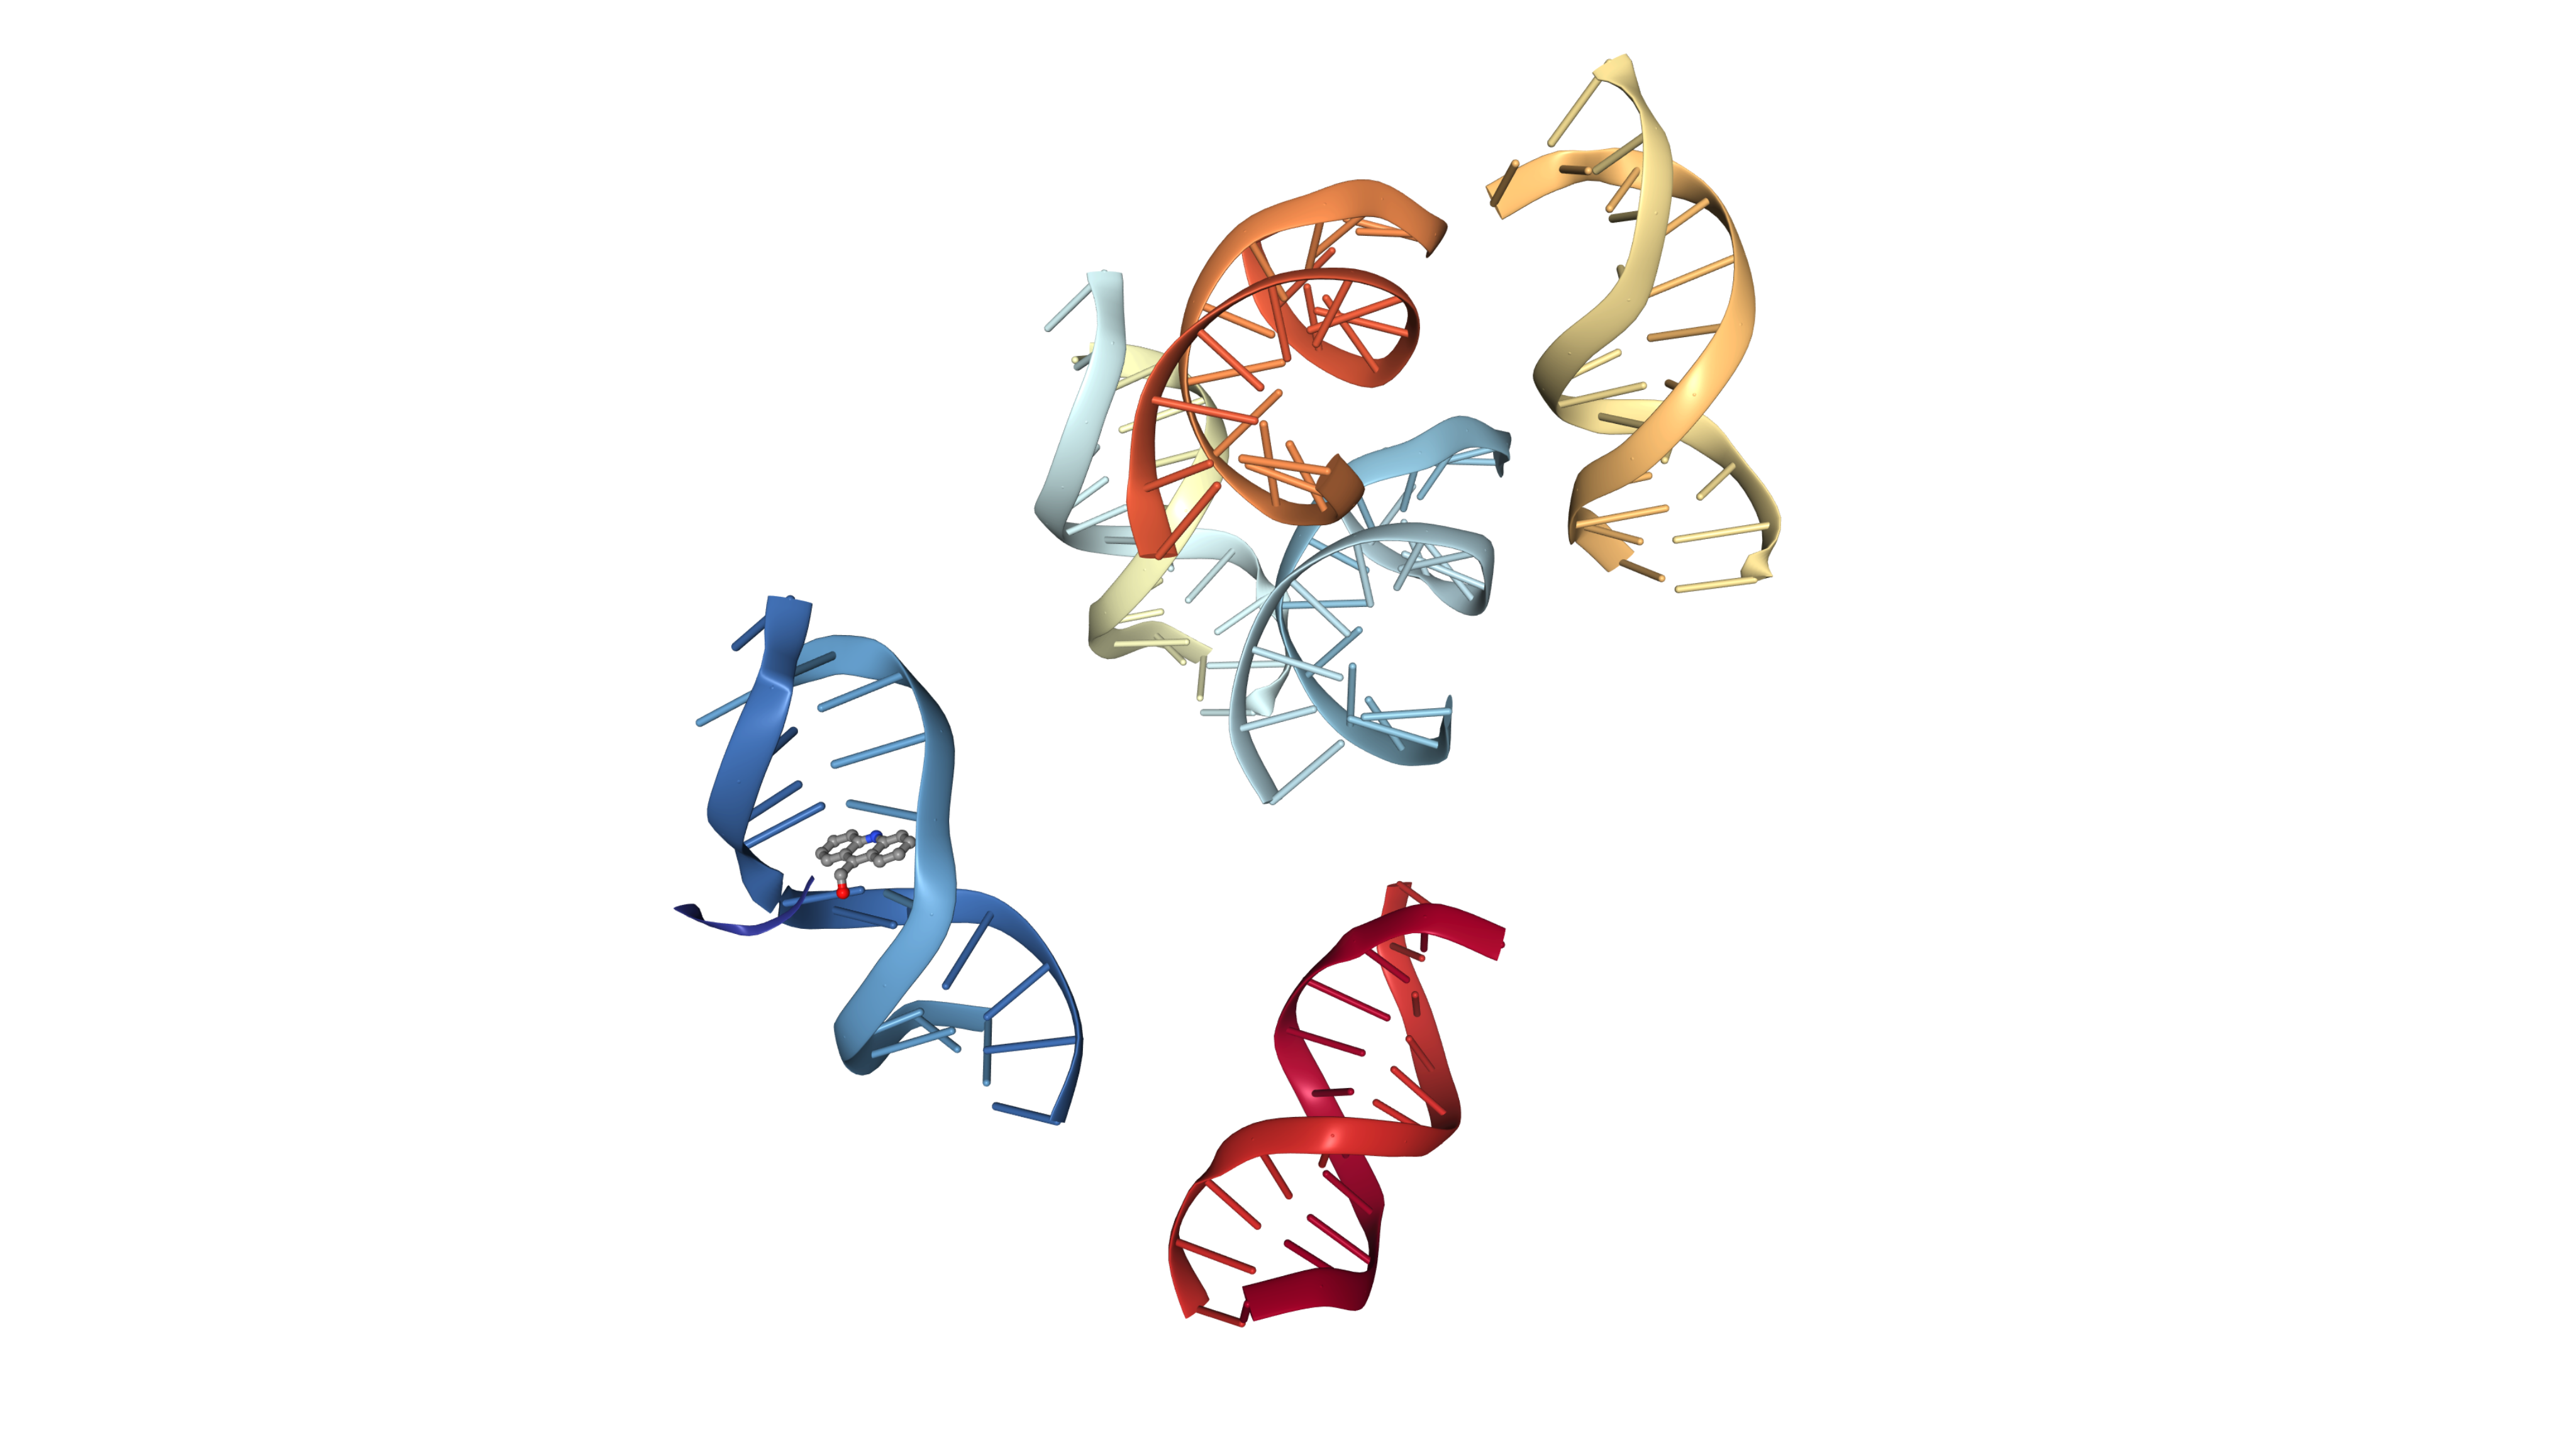
\includegraphics[width=\textwidth]{1g3x.png}
  \caption{Raw PDB structure from database. Contains 6 strands in unit cell. Needs processing.}
  \label{fig:pdb-1}
\end{figure}

\begin{figure}
  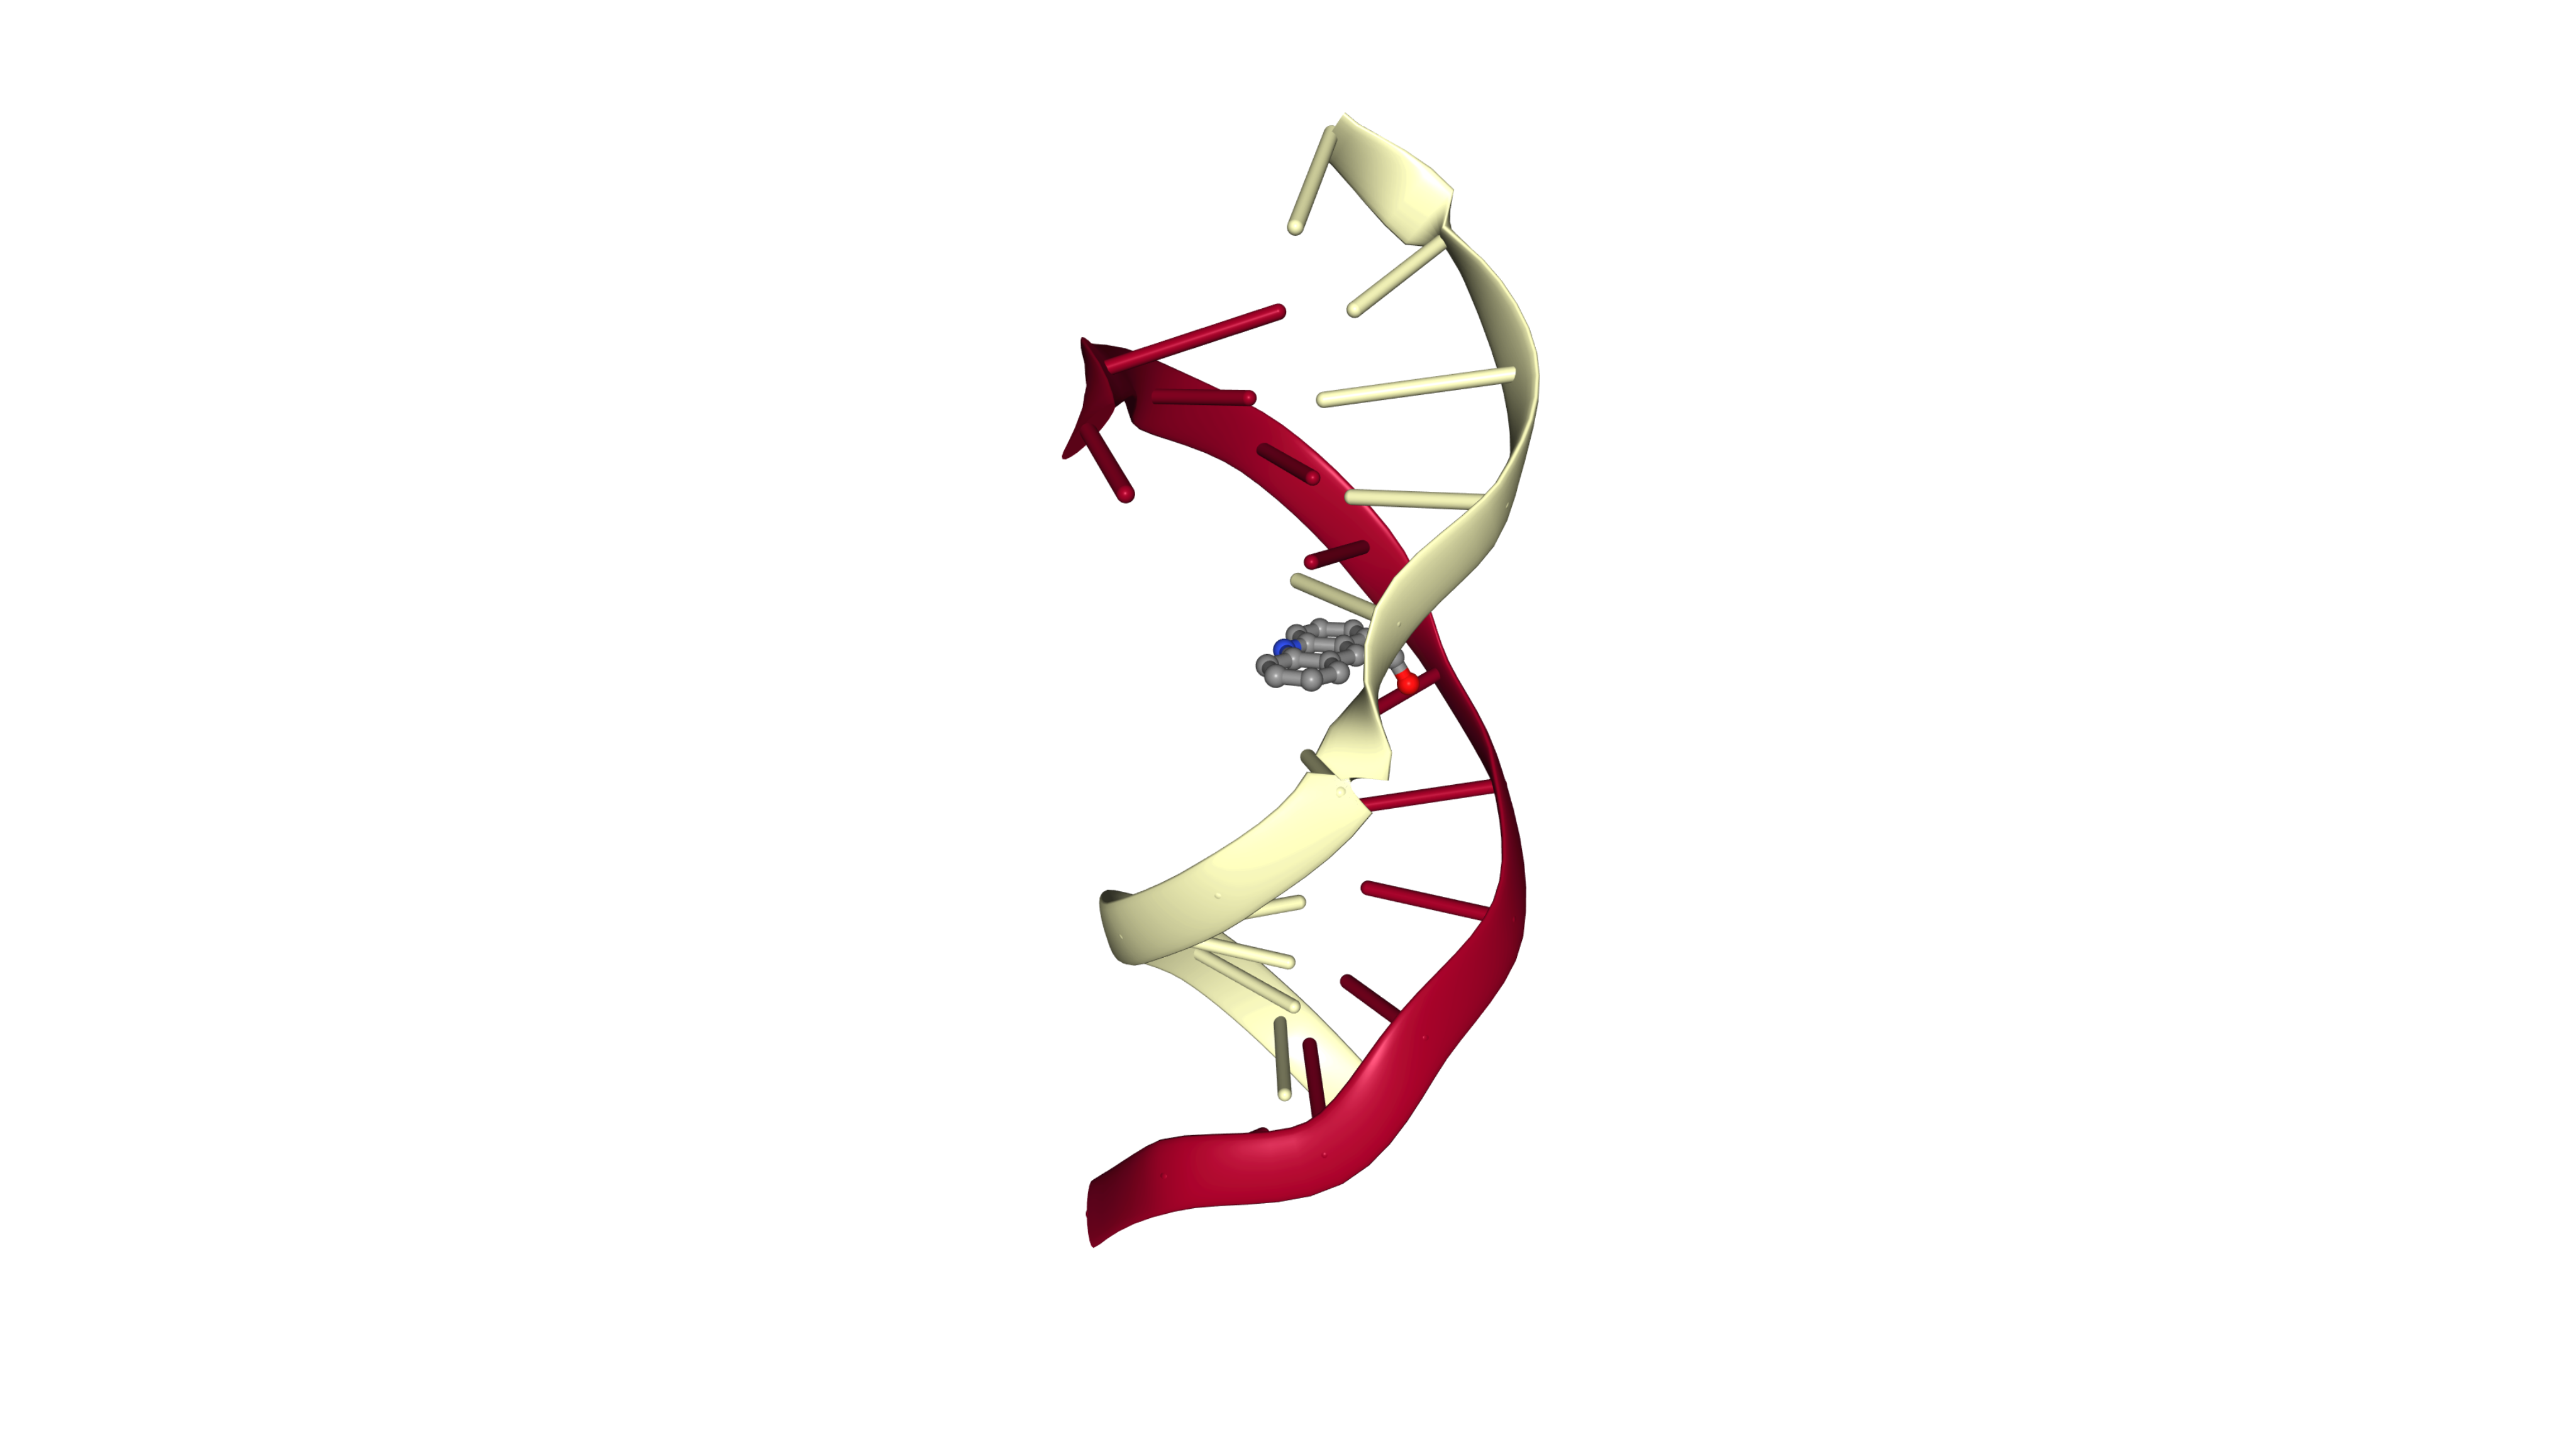
\includegraphics[width=\textwidth]{1g3x_clean.png}
  \caption{Processed DNA to be simulated. Stripped additional strands, and removed ions and water. This will be added later during the parametrisation step.}
  \label{fig:pdb-2}
\end{figure}

\begin{figure}
  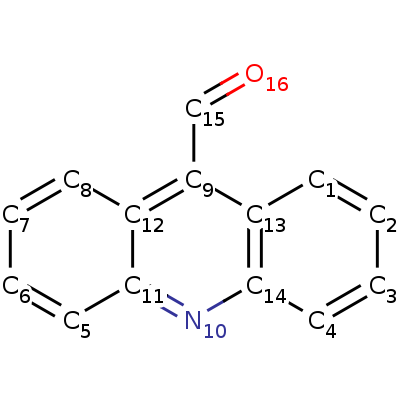
\includegraphics[width=\textwidth]{9AC-large.png}
  \caption{The intercalator molecule. A planar aromatic compound. Charges will be assigned with AM1BCC method and parametrisation with the General Amber Force Field 2.}
  \label{fig:pdb-3}
\end{figure}

\end{document}
